\documentclass[11pt]{article}
\usepackage[margin=1.1in]{geometry}
\usepackage{amsmath}
\usepackage{graphicx}
\usepackage{booktabs}

\usepackage[hidelinks]{hyperref}
\renewcommand{\labelitemi}{$\bullet$}

\title{Measuring and Removing an Object's Light Footprint:\\
\large Reflection-Aware Object Removal in 3D Gaussian Splatting via Render--Edit--Refit}
\author{Yonghao Lee\\[2pt]
{\normalsize Deep Learning for 3D Computer Vision --- Final Report}\\
{\normalsize Hebrew University of Jerusalem \quad $\cdot$ \quad Instructor: Sagie Benaim}}
\date{September 2026}

\begin{document}
\maketitle

\begin{abstract}
Deleting an object from a reconstructed 3D Gaussian Splatting (3DGS) scene removes its geometry but not its light footprint: the shadow it casts, its image in nearby mirrors, and the colour it bleeds onto surrounding surfaces all survive as painted-on texture. We study whether a pretrained video prior can remove this footprint through a simple \emph{render--edit--refit} pipeline: render an orbit from the fitted scene, edit the video with a diffusion prior, and re-fit a fresh 3DGS on the edited frames. To measure the problem exactly, we built a synthetic benchmark in which the same camera path is rendered with and without the object, giving pixel-exact clean plates and automatically derived footprint regions. Our central negative finding is that a strong generalist editor (VACE) does not remove: it \emph{substitutes}, replacing the masked object with a new one --- and, given only the object mask, it reconstructs the object from its own shadow and reflection. A removal-specialised prior (ROSE) with masks covering the footprint behaves differently: footprint-region PSNR improves from 14.2\,dB (deletion) to 28.4\,dB. The masks need not be oracles --- four clicks on a single frame, propagated by SAM~2, match oracle-mask performance (31.3 vs.\ 31.1\,dB full-frame). Finally, the edits survive the lift back to 3D: all numbers are measured on held-out novel views rendered from the re-fitted scene, without any explicit multi-view consistency mechanism.
\end{abstract}

\section{Introduction}
Imagine a red vase standing on a polished floor in front of a wall mirror. A 3D reconstruction of this room --- here, a 3D Gaussian Splatting model \cite{kerbl3dgs} --- stores the vase's geometry, but it also stores everything the vase \emph{does to the light}: the shadow it casts on the floor, its image in the mirror, the faint red glow it bleeds onto the wall. Formally, the radiance the scene records is
\[
L \;=\; L_{\mathrm{direct}} \;+\; L_{\mathrm{obj}},
\]
where $L_{\mathrm{obj}}$ collects every contribution that exists only because the object does. Removing the object's Gaussians deletes the first-order geometry but leaves $L_{\mathrm{obj}}$ baked into the surrounding surfaces --- a shadow with no caster, a reflection with no source. The goal of this project is to remove the object \emph{together with} its light footprint, consistently across viewpoints, and to measure exactly how much of the footprint each method removes.

Our approach is deliberately simple: rather than reasoning about light transport inside the 3D representation, we render a smooth orbit from the fitted scene, hand the video to a pretrained video diffusion prior that has seen millions of examples of scenes with and without objects, and re-fit a fresh 3DGS on the edited frames. The scientific question is whether such a prior actually knows how to \emph{remove} --- and whether per-frame edits survive the lift back to 3D.

Our contributions are:
\begin{enumerate}
  \item \textbf{A controlled benchmark} with pixel-exact clean plates and automatically derived footprint regions, obtained by rendering the same camera path with and without the object (Section~\ref{sec:benchmark}).
  \item \textbf{A render--edit--refit pipeline} for footprint-aware object removal that requires no COLMAP, no model training, and no architecture changes (Section~\ref{sec:method}).
  \item \textbf{An empirical study of video priors as removers}, with a clear negative result: a generalist editor substitutes rather than removes, to the point of rebuilding the object from its own footprint (Section~\ref{sec:substitution}).
  \item \textbf{A practical annotation protocol}: four clicks on one frame, propagated by SAM~2, match oracle footprint localization (Section~\ref{sec:practical}).
\end{enumerate}

\section{Related Work}
\paragraph{Object removal and 3D inpainting.}
Removal from radiance fields is usually cast as segmentation plus inpainting: SPIn-NeRF \cite{spinnerf} lifts multiview masks and inpaints with a 2D prior; Weder et al.\ \cite{weder} learn view-consistent inpainting confidence; OR-NeRF \cite{ornerf} propagates user clicks with SAM \cite{sam}. In the 3DGS setting, GScream \cite{gscream} and Gaussian Grouping \cite{gaussiangrouping} segment and delete Gaussians before repairing the hole. These methods focus on the hole the object leaves in geometry; the footprint on \emph{other} surfaces is out of scope.

\paragraph{Footprint-aware removal.}
GauComp \cite{gaucomp} and GOR-IS \cite{goris} explicitly target associated shadows during Gaussian removal, and full inverse rendering such as IRGS \cite{irgs} would in principle explain reflections physically, at substantial cost in scene assumptions. Kuchler et al.\ \cite{lighting} ask whether 2D editing models understand lighting at all. Our pipeline is representation-agnostic: all lighting reasoning is delegated to a video prior.

\paragraph{Measuring what removal leaves behind.}
SPIn-NeRF's paired evaluation scenes and, most directly, Remove360 \cite{remove360,semanticresiduals} established that removal quality must be measured against ground truth \emph{after} removal, and that residuals can remain semantically revealing. We follow this philosophy but move it to synthetic scenes where clean plates are pixel-exact and footprint regions are derived automatically rather than annotated.

\paragraph{Diffusion-based 3D editing.}
Instruct-NeRF2NeRF \cite{in2n} and Instruct-GS2GS \cite{igs2gs} alternate 2D edits (with InstructPix2Pix \cite{ip2p}) and 3D re-optimisation to keep multi-view consistency. Our pipeline is the degenerate one-round version: edit once, re-fit once; Section~\ref{sec:consistency} measures whether that suffices.

\paragraph{Video diffusion priors.}
VACE \cite{vace} is a strong general video creation-and-editing model; ROSE \cite{rose} is fine-tuned specifically to remove objects \emph{with their side effects} (shadows, reflections) within a single 2D video; $\int$-noise \cite{warpnoise} offers temporally consistent noise for video diffusion. ROSE removes side effects within a single 2D video; we study whether such a prior can remove them from a 3D \emph{scene}, and measure what survives the lift back to 3D. SAM~2 \cite{sam2} supplies the mask propagation for our practical protocol.

To our knowledge, no prior work provides a controlled benchmark that measures, per physical effect and in 3D, what object removal leaves behind --- the gap this project addresses.

\section{Benchmark}
\label{sec:benchmark}
The benchmark is one compact Blender/Cycles scene --- a red sphere on a floor, a white wall, and a wall mirror --- rendered along an 81-frame, $120^\circ$ camera arc at $832{\times}480$, twice: once with the object and once without, with identical cameras and lighting (Figure~\ref{fig:dataset}). The design of the scene is the result of iterating against an explicit checklist (every footprint effect must be visible to the eye in the renders), and several choices carry the lessons of that iteration:

\begin{itemize}
  \item \textbf{Polished dielectric floor, not a metallic mirror floor.} Our first floor was metallic: it produced a beautiful reflection and \emph{no visible shadow}, because a pure specular surface has no diffuse response for a shadow to darken. A glossy dielectric floor shows both a soft reflection and a clear shadow.
  \item \textbf{A separate vertical mirror panel.} At our viewing angles, dielectric Fresnel reflection on the floor is too weak to serve as the headline mirror effect; a dedicated mirror gives the footprint a second, unambiguous component.
  \item \textbf{A fill light.} A mirror faithfully shows the \emph{unlit} side of the object; without a fill light the mirror image is a dark, unrecognisable blob.
  \item \textbf{Shared cameras $\Rightarrow$ exact clean plates.} Because the with/without renders share every camera, the without-render \emph{is} the ground-truth answer to ``what should removal produce?'' --- no inpainting benchmark ambiguity. Differencing the two renders outside the object silhouette yields per-region footprint masks (shadow, mirror image, floor reflection, wall bleed) with no manual annotation.
  \item \textbf{$832{\times}480$, 81 frames.} This matches the native resolution of the video models we evaluate and satisfies their $16n{+}1$ frame-count constraint, so the editor never resamples our data.
  \item \textbf{Every 8th frame held out.} All metrics in this report are computed on the 11 held-out views, rendered from a re-fitted 3DGS --- novel-view quality, not training-view quality. We note honestly that these views interpolate the arc; extrapolation far off the arc is not measured.
\end{itemize}

\begin{figure}[t]
  \centering
  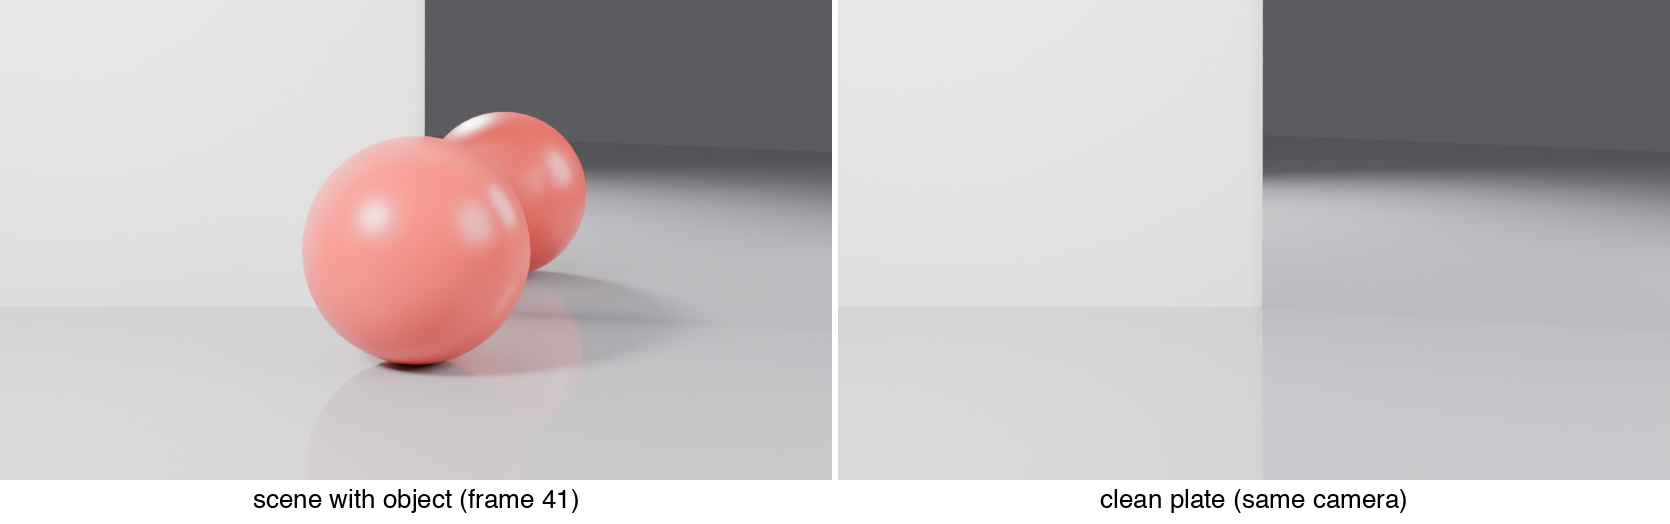
\includegraphics[width=\linewidth]{figures/fig1_dataset_pair.png}
  \caption{The benchmark pair at mid-arc. Left: scene with the object --- note the four footprint components (shadow, mirror image, floor reflection, and a faint red bleed on the wall). Right: the exact clean plate from the same camera.}
  \label{fig:dataset}
\end{figure}

\section{Method: Render--Edit--Refit}
\label{sec:method}
The pipeline has four steps, none of which trains or modifies a model.

\textbf{Step 1 --- Reconstruct.} We fitted \texttt{splatfacto} (nerfstudio's 3DGS) for 15{,}000 iterations on the 70 training frames of the with-object renders. Because the poses are exact and the scene is bounded, we used random point initialisation rather than an SfM point cloud, following the original 3DGS finding that synthetic bounded scenes tolerate random init \cite{kerbl3dgs}; this also removes COLMAP from the pipeline entirely.

\textbf{Step 2 --- Render an orbit.} From the fitted scene we rendered all 81 poses of the arc. In the general (real-scene) case this step is what buys exact known poses for every edited frame; in our benchmark the poses are known anyway, which lets us validate the pipeline itself.

\textbf{Step 3 --- Edit the video.} A pretrained video diffusion prior edits the orbit under a binary mask video (white $=$ edit, black $=$ keep). We evaluate two editors: VACE (Wan2.1-VACE-1.3B \cite{vace}; 30 denoising steps, guidance 5.0, seeded, VAE kept at fp32 to avoid colour banding), prompted with a description of the \emph{target} state (``an empty room \dots\ nothing on the floor'') and a negative prompt naming the footprint effects; and ROSE \cite{rose} (Wan2.1-Fun-1.3B-InP base with the ROSE fine-tuned transformer, 50 steps), which takes only video~$+$~mask.

Three mask protocols are compared, stated precisely:
\begin{itemize}
  \item \textbf{Object mask}: the object silhouette (from the renderer's object index pass; in a real scene, SAM), dilated by 25\,px.
  \item \textbf{Oracle mask}: all pixels that differ between the with/without renders --- object \emph{and} footprint --- dilated by 15\,px. This uses ground truth and is labelled an upper bound.
  \item \textbf{Practical mask}: four clicks on one frame propagated by SAM~2 across all 81 frames, unioned and dilated by 15\,px (Section~\ref{sec:practical}).
\end{itemize}

\textbf{Step 4 --- Re-fit.} A fresh \texttt{splatfacto} is trained on the edited frames with the \emph{unchanged} poses, using the identical recipe as Step~1 (15k iterations, random init). No keep-loss or masking is applied at re-fit; unedited-region fidelity is therefore captured by the full-frame metric.

\section{Experiments}
All quantitative results are PSNR against the exact clean plates on the 11 held-out views, full-frame and restricted to the ground-truth footprint region, always after re-fitting a fresh 3DGS on the edited frames (Table~\ref{tab:main}).

\subsection{Reconstruction quality (ceiling)}
The Step-1 reconstruction reaches \textbf{45.7\,dB} PSNR (0.992 SSIM, 0.021 LPIPS) on held-out views of the with-object scene (Figure~\ref{fig:recon}). This matters for attribution: reconstruction error is negligible at the scale of every effect we measure below, so any later degradation is caused by removal, not by 3DGS fitting.

\begin{figure}[t]
  \centering
  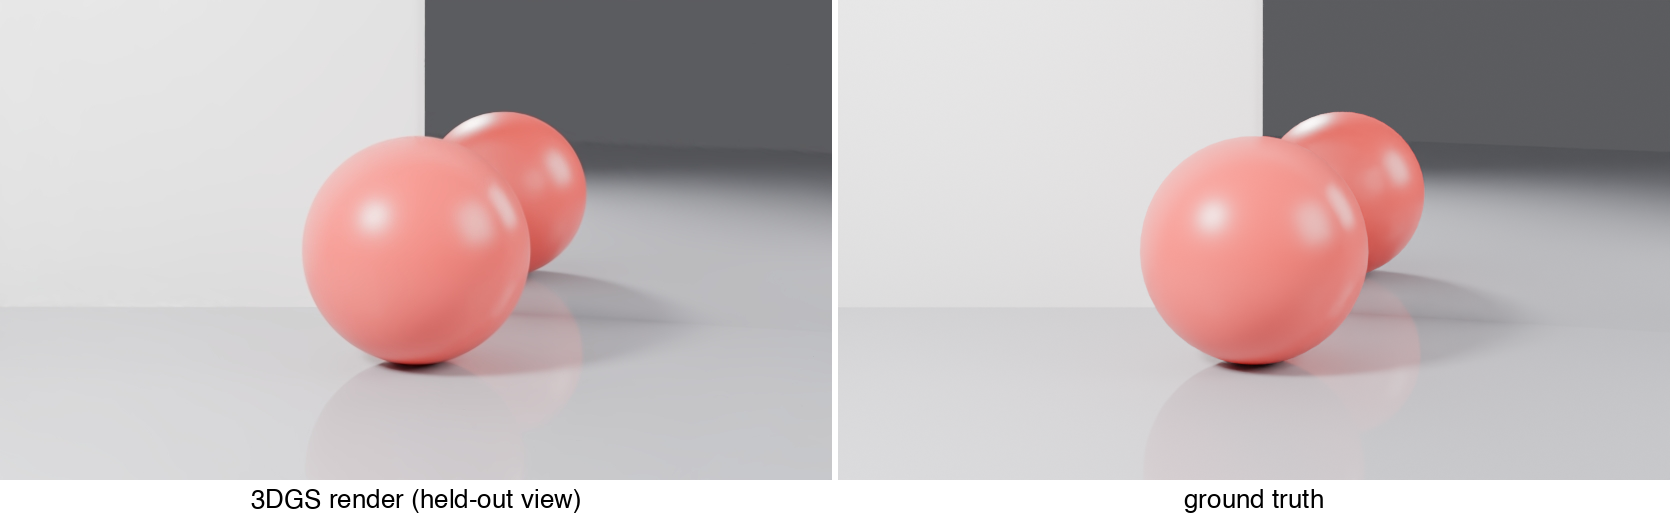
\includegraphics[width=\linewidth]{figures/fig2_recon_vs_gt.png}
  \caption{Reconstruction ceiling: a held-out view rendered from the fitted 3DGS (left) against ground truth (right) --- visually indistinguishable at 45.7\,dB.}
  \label{fig:recon}
\end{figure}

\subsection{The problem, quantified (M1: deletion)}
The deletion baseline selects the object's Gaussians by lifting the 2D object masks: a Gaussian is selected if its center projects inside the mask in ${\geq}90\%$ of the views that see it (${\geq}40$ views). Validated against the ground-truth sphere geometry, the 2{,}888 selected Gaussians achieve 100\% precision and 90\% recall; the missed 10\% are 318 interior Gaussians invisible from outside, which the geometric check adds to the deletion set. Deletion then does exactly what it promises: the sphere is gone, and its mirror image, shadow, and floor reflection remain, intact and sharp (Figure~\ref{fig:ghost}). Quantitatively: 23.1\,dB full-frame, \textbf{14.2\,dB} in the footprint --- the number the rest of the paper tries to raise.

\begin{figure}[t]
  \centering
  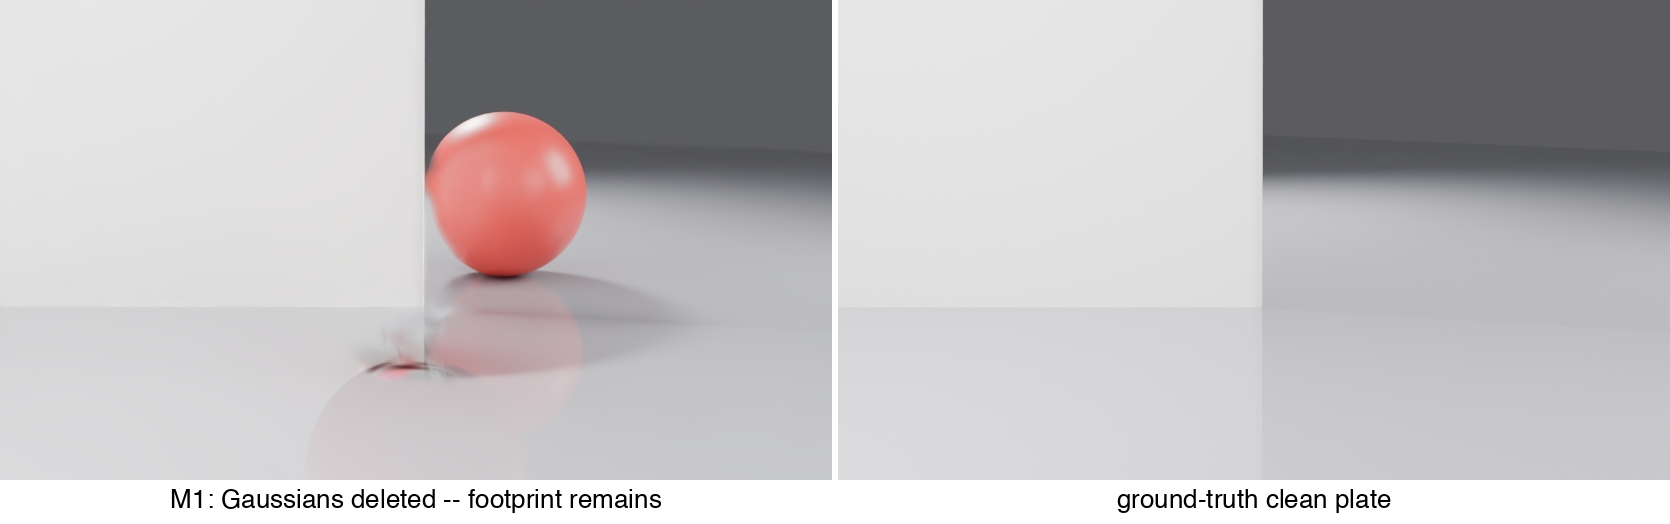
\includegraphics[width=\linewidth]{figures/fig3_ghost.png}
  \caption{The ghost. Left: held-out view rendered after deleting the object's Gaussians --- a mirror image with no object, a shadow with no caster. Right: ground-truth clean plate.}
  \label{fig:ghost}
\end{figure}

\subsection{Main results}
\begin{table}[h]
\centering
\begin{tabular}{lcc}
\toprule
Method & PSNR full & PSNR footprint \\
\midrule
Reconstruction ceiling            & 45.7 & --   \\
M1: Gaussian deletion             & 23.1 & 14.2 \\
M3: VACE, object mask             & 21.6 & 14.2 \\
M3: VACE, oracle mask             & 18.2 & 13.1 \\
M3: ROSE, object mask             & 23.2 & 15.0 \\
M3: ROSE, oracle mask             & 31.1 & 28.4 \\
M3: ROSE, SAM2 masks (4 clicks)   & \textbf{31.3} & \textbf{28.4} \\
\bottomrule
\end{tabular}
\caption{PSNR (dB) vs.\ exact clean plates on held-out novel views, full-frame
and restricted to ground-truth footprint regions. All rows measured after
re-fitting a fresh 3DGS on the edited frames.}
\label{tab:main}
\end{table}

Walking the table: the two VACE rows sit at or \emph{below} deletion --- the generalist prior actively hurts (Section~\ref{sec:substitution} shows why). ROSE with the object mask barely moves the footprint number (15.0\,dB): the specialised prior deletes cleanly inside its mask but touches nothing outside it, so masking --- not the prior --- is the bottleneck. Giving ROSE a mask that covers the footprint changes the regime: 28.4\,dB in the footprint, a \textbf{$+$14.2\,dB} gain over deletion, and 31.1\,dB full-frame. The final row is the practical protocol: four clicks match the oracle (31.3/28.4), which is the operationally important result --- oracle-quality localization costs a user seconds, not ground truth. As the benchmark is new, there are no published numbers to cite for it; deletion (M1) is the natural baseline all rows share.

\subsection{Why the generalist prior fails: substitution, not removal}
\label{sec:substitution}
VACE's failure is systematic and instructive (Figure~\ref{fig:vace}). Given the \emph{object mask}, it filled the hole with a gray sphere --- reconstructing the object it was asked to delete from the evidence left \emph{outside} the mask: the shadow and reflections. This is direct visual evidence that the footprint encodes the object, the physical-scene counterpart of Remove360's finding that residuals remain semantically revealing \cite{semanticresiduals}. Given the \emph{oracle mask} (footprint included), it substituted a cyan sphere --- and rendered a \emph{matching cyan reflection} in the mirror. The prior evidently understands object--reflection coupling; what it lacks is ``generate emptiness'' as an operation. Prompting cannot override the mask's shape prior: across three prompt variants, including an emptiness-dominant prompt at raised guidance, we obtained three different objects (gray, cyan, orange) and zero removals. We conclude that the masked region's shape acts as a strong object prior for a generation-trained model, and removal requires a prior trained for removal.

\begin{figure}[t]
  \centering
  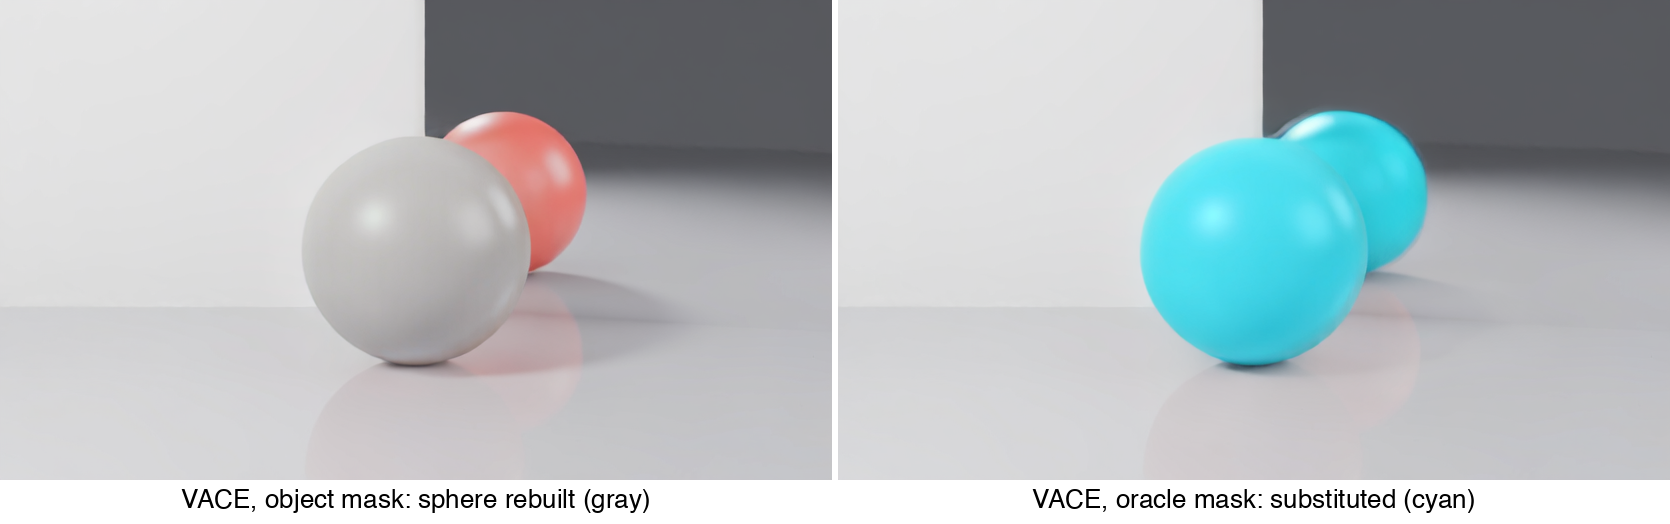
\includegraphics[width=\linewidth]{figures/fig4_vace_substitution.png}
  \caption{Substitution, not removal. Left: VACE with the object mask rebuilds the sphere (gray) from its own shadow and reflections. Right: with the oracle mask it substitutes a cyan sphere --- with a physically coherent cyan mirror image. A third, emptiness-dominant prompt produced an orange sphere (not shown).}
  \label{fig:vace}
\end{figure}

\begin{figure}[t]
  \centering
  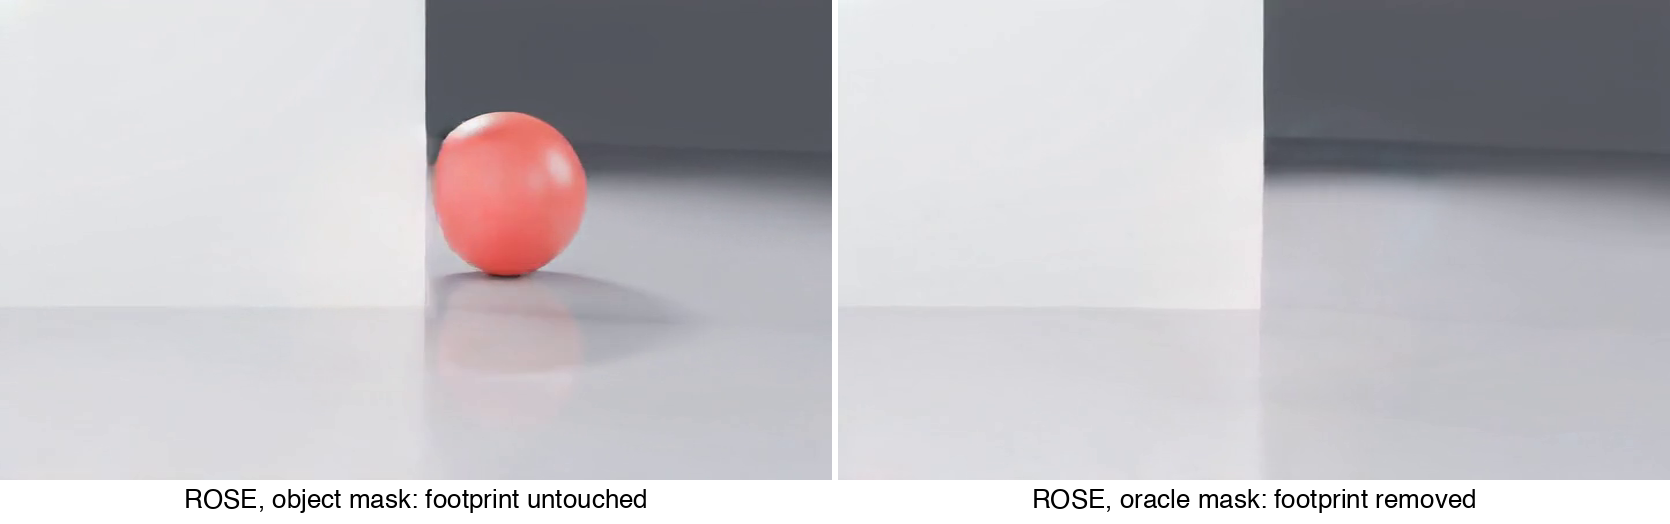
\includegraphics[width=\linewidth]{figures/fig5_rose_obj_vs_oracle.png}
  \caption{ROSE is mask-limited, not prior-limited. Left: object mask --- the sphere is removed cleanly but its mirror image and shadow survive untouched outside the mask. Right: oracle mask --- object and footprint removed together.}
  \label{fig:rose}
\end{figure}

\subsection{Multi-view consistency of independent edits}
\label{sec:consistency}
The proposal reserved two remedies for cross-view inconsistency of per-frame edits: iterative dataset update in the style of Instruct-GS2GS \cite{igs2gs}, and warped noise \cite{warpnoise}. The experiment resolved the question by measurement instead: ROSE edits all 81 frames of the orbit as a video but with no knowledge of our 3D scene, yet the re-fit on those frames reaches 31.3\,dB on held-out views --- above the edited-region quality that either remedy could plausibly rescue. At this operating point, the 3D representation itself absorbs the residual frame-to-frame disagreement, averaging it into a slightly soft but consistent scene. One honest caveat: at lower edit quality (e.g.\ VACE's substitutions, which flicker in identity across frames) consistency machinery might still matter; we did not need it where it would have helped, and it could not have helped where we needed it.

\subsection{The practical protocol}
\label{sec:practical}
The oracle mask uses ground-truth differencing, unavailable in any real scene. The practical protocol replaces it with four clicks on the middle frame of the orbit --- one each on the sphere, its mirror image, its shadow, and its floor reflection (Figure~\ref{fig:clicks}) --- propagated bidirectionally across all 81 frames by SAM~2.1, unioned and dilated by 15\,px (Figure~\ref{fig:sam2}). Two observations from running it: shadows and floor sheen are outside SAM~2's comfort zone --- the propagated regions drift over the arc --- but the union over four regions plus dilation absorbs the drift; and the wall colour bleed was too faint to click at all, yet did not measurably hurt the score. The protocol ties the oracle (31.3 vs.\ 31.1\,dB full-frame, 28.4\,dB footprint in both cases), and the final result is an empty room whose mirror shows an empty room (Figure~\ref{fig:final}).

\begin{figure}[t]
  \centering
  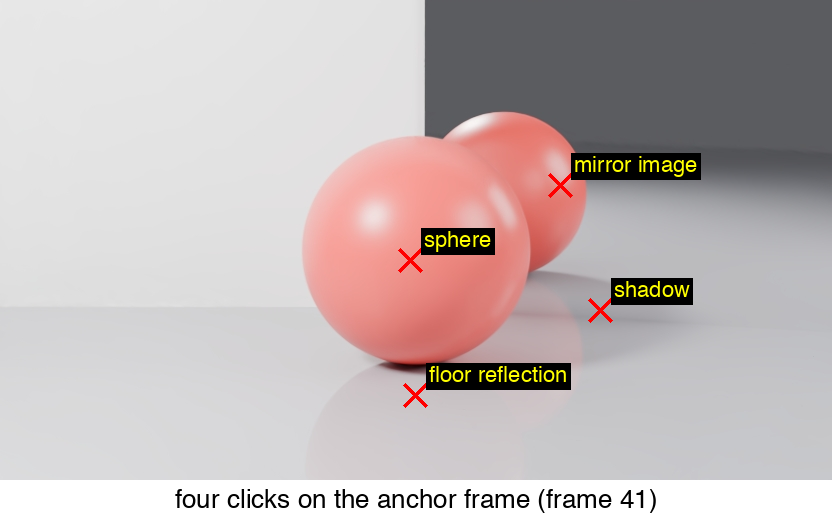
\includegraphics[width=0.72\linewidth]{figures/fig6_annotation_clicks.png}
  \caption{The entire annotation budget: four clicks on one frame.}
  \label{fig:clicks}
\end{figure}

\begin{figure}[t]
  \centering
  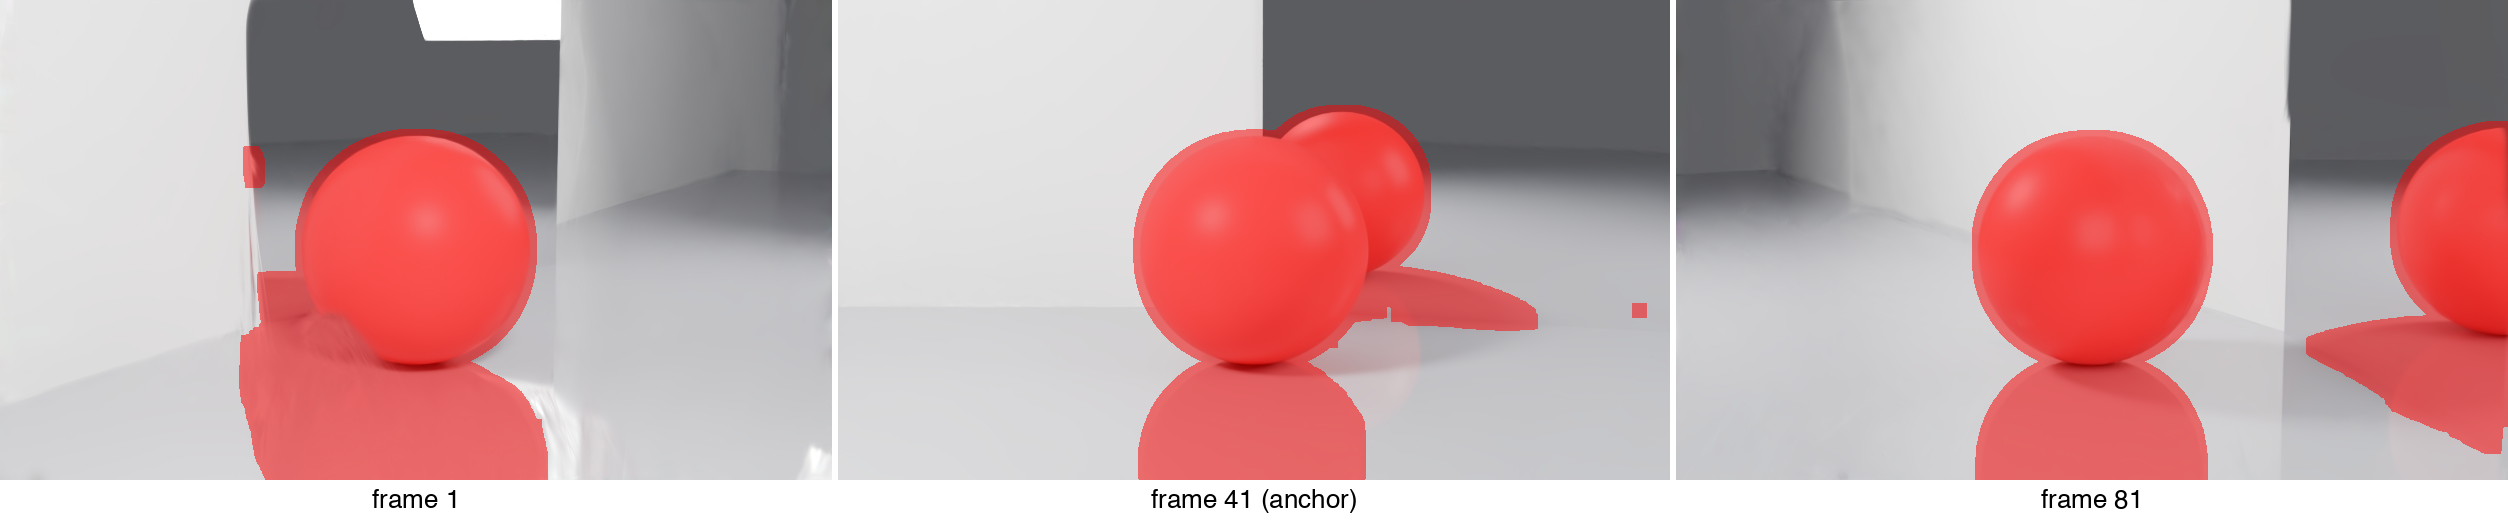
\includegraphics[width=\linewidth]{figures/fig7_sam2_masks.png}
  \caption{SAM~2 propagation of the four clicked regions (red overlay) at the start, anchor, and end of the arc.}
  \label{fig:sam2}
\end{figure}

\begin{figure}[t]
  \centering
  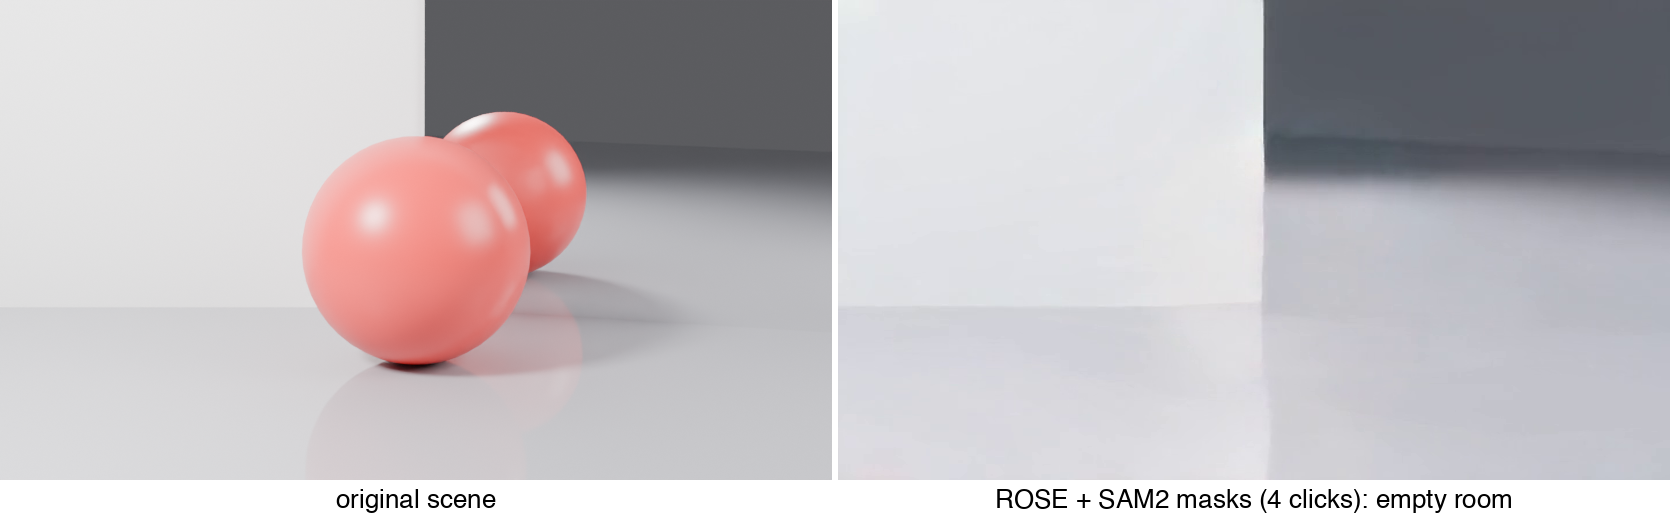
\includegraphics[width=\linewidth]{figures/fig8_final_pair.png}
  \caption{The headline result. Left: original scene. Right: ROSE with the 4-click SAM~2 masks --- object, shadow, mirror image, and floor reflection all removed (31.3\,dB on held-out novel views after re-fitting).}
  \label{fig:final}
\end{figure}

\section{Limitations and Lessons}
This study is deliberately narrow, and its limitations should be stated plainly. Everything is measured on a single synthetic scene with a single object; the camera arc spans $120^\circ$, so held-out views interpolate rather than extrapolate. The re-fit uses no keep-loss, so unedited regions may drift --- bounded, however, by the full-frame PSNR, which sits within 0.2\,dB of the footprint-driven gap. The oracle masks use ground truth, though the practical protocol matching them largely defuses this concern. Our metrics combine all footprint effects into one region; the per-effect masks (shadow vs.\ mirror image vs.\ bleed) already exist as a by-product of the differencing and splitting the table by effect is mechanical future work, as is adding SSIM/LPIPS to the removal rows (currently reported for the ceiling only) and a qualitative real-capture demo. The proposal's in-context-examples extension (conditioning the editor on a Blender before/after pair) was not run: it was designed to teach a generalist prior what removal means, and adopting ROSE --- a prior already trained for exactly that --- made it moot; we report this as a descoped promise rather than a finding.

Two engineering lessons survived contact with the infrastructure: pin dependency versions inside every notebook (a transformers upgrade silently broke ROSE's loader mid-project), and when an experiment looks absurd, verify \emph{which inputs actually reached the model} before theorising --- our first ``VACE ignores the mask'' hypothesis was in fact a mask-video encoding bug.

\section{Conclusion}
Removing an object from a 3DGS scene together with its light footprint can be done without touching the 3D representation's internals: render an orbit, edit it with a removal-specialised video prior under masks that cover the footprint, and re-fit --- raising footprint-region PSNR from 14.2\,dB to 28.4\,dB over deletion, with 31.3\,dB full-frame on held-out novel views and no explicit consistency machinery. The equally important negative result is that a strong generalist video editor cannot do this: it substitutes objects rather than removing them, and will happily rebuild an object from its own shadow. The benchmark --- paired with/without renders, exact clean plates, derived footprint masks --- is released with all scripts and notebooks at the project repository, and is, we believe, the right instrument for the next question: which physical effect (shadow, reflection, bleed) survives which remover.

\section*{Contribution Statement}
All experiments and writing are by the author (solo project). Coding assistance and debugging support were provided by an AI assistant (Claude); all code was reviewed and all results verified by the author. Third-party models and libraries (nerfstudio, VACE, ROSE, SAM~2) are used as released, unmodified.

\begin{thebibliography}{20}
\bibitem{kerbl3dgs} B. Kerbl, G. Kopanas, T. Leimk\"uhler, G. Drettakis. \emph{3D Gaussian Splatting for Real-Time Radiance Field Rendering}. SIGGRAPH 2023.
\bibitem{spinnerf} A. Mirzaei et al. \emph{SPIn-NeRF: Multiview Segmentation and Perceptual Inpainting with NeRF}. CVPR 2023.
\bibitem{weder} S. Weder et al. \emph{Removing Objects From Neural Radiance Fields}. CVPR 2023.
\bibitem{ornerf} Y. Yin, Z. Fu, F. Yang, G. Lin. \emph{OR-NeRF: Object Removing from 3D Scenes Guided by Multiview Segmentation with NeRF}. arXiv 2023.
\bibitem{gscream} Y. Wang, Q. Wu, G. Zhang, D. Xu. \emph{GScream: Learning 3D Geometry and Feature Consistent Gaussian Splatting for Object Removal}. ECCV 2024.
\bibitem{gaussiangrouping} M. Ye, M. Danelljan, F. Yu, L. Ke. \emph{Gaussian Grouping: Segment and Edit Anything in 3D Scenes}. ECCV 2024.
\bibitem{sam} A. Kirillov et al. \emph{Segment Anything}. ICCV 2023.
\bibitem{gaucomp} W. Zheng, Y. Li, J. Xiang, X. Peng, C. Wang. \emph{GauComp: 3D Gaussian Completion for Associated Shadow and Object Removal}. Computer Graphics Forum 2026.
\bibitem{goris} Y. Zhao, Y. Gao, J. Yang, J. Xie, B. Wang. \emph{GOR-IS: 3D Gaussian Object Removal in the Intrinsic Space}. arXiv 2026.
\bibitem{in2n} A. Haque, M. Tancik, A. Efros, A. Holynski, A. Kanazawa. \emph{Instruct-NeRF2NeRF: Editing 3D Scenes with Instructions}. ICCV 2023.
\bibitem{igs2gs} C. Vachha, A. Haque. \emph{Instruct-GS2GS: Editing 3D Gaussian Splats with Instructions}. 2024. \texttt{instruct-gs2gs.github.io}.
\bibitem{vace} Z. Jiang, Z. Han, C. Mao, J. Zhang, Y. Pan, Y. Liu. \emph{VACE: All-in-One Video Creation and Editing}. ICCV 2025.
\bibitem{remove360} S. Kocour, A. Benbihi, T. Sattler. \emph{Remove360: Benchmarking Residuals After Object Removal in 3D Gaussian Splatting}. arXiv 2025.
\bibitem{semanticresiduals} S. Kocour, A. Benbihi, A. Adam, T. Sattler. \emph{Is There Anything Left? Measuring Semantic Residuals of Objects Removed from 3D Gaussian Splatting}. arXiv 2025.
\bibitem{irgs} C. Gu, X. Wei, Z. Zeng, Y. Yao, L. Zhang. \emph{IRGS: Inter-Reflective Gaussian Splatting with 2D Gaussian Ray Tracing}. arXiv 2024.
\bibitem{ip2p} T. Brooks, A. Holynski, A. Efros. \emph{InstructPix2Pix: Learning to Follow Image Editing Instructions}. CVPR 2023.
\bibitem{warpnoise} P. Chang, J. Tang, M. Gross, V. C. Azevedo. \emph{How I Warped Your Noise: a Temporally-Correlated Noise Prior for Diffusion Models}. ICLR 2024 (oral).
\bibitem{rose} C. Miao et al. \emph{ROSE: Remove Objects with Side Effects in Videos}. arXiv 2025.
\bibitem{sam2} N. Ravi et al. \emph{SAM 2: Segment Anything in Images and Videos}. arXiv 2024.
\bibitem{lighting} T. Kuchler, J.-F. Feiden, M. Nie{\ss}ner, C. Rother. \emph{Do Image Editing Models Understand Lighting?} 2026.
\end{thebibliography}

\end{document}
